\documentclass[../main]{subfiles}
\begin{document}

\chapter{实验概述}%
\label{cha:introduction}

学生实验用小型雷达系统(以下简称“教学雷达”)在电子与信息工程专业
《雷达原理》\cite{丁鹭飞2009雷达原理}的教学中具有重要的地位,在教学大纲和学生
的培养计划中起到关键作用,是课程实验重要的实验装置。

通过实验,学生能够把传统的教学方法和现代的教学方法相结合。学生通过接触实验用
小型雷达系统能够提高自身将雷达理论与具体雷达系统结合的能力,激发学生学习雷达
的热情和求知欲,加深对雷达系统的理解和记忆,帮助引发学生进一步的思考,潜移默
化地提升学生的逻辑思维能力、自主实践能力、科技创新能力。

\section{基本信息}%
\label{sec:information}

\subsection{实验名称}%
\label{sub:name}

雷达原理课程(3.5 学分)课内实验。

\subsection{实验时间}%
\label{sub:time}

\today,8:00--12:00

\subsection{实验场地}%
\label{sub:spot}

如图~\ref{fig:spot},南京理工大学电光学院院办东侧道路,约东经\ang{118;51;29},
北纬\ang{32;1;36}。

\begin{figure}[htbp]
  \centering
  \begin{subfigure}[htbp]{0.45\linewidth}
    \centering
    \includegraphics[
    width = \linewidth,
    ]{spot/map}
    \caption{地图}%
    \label{fig:spot/map}
  \end{subfigure}
  \quad
  \begin{subfigure}[htbp]{0.45\linewidth}
    \centering
    \includegraphics[
    width = 0.3\linewidth,
    ]{spot/position}
    \caption{经纬度}%
    \label{fig:spot/position}
  \end{subfigure}
  \caption{实验场地}%
  \label{fig:spot}
\end{figure}

\subsection{实验仪器}%
\label{sub:instrument}

见表~\ref{tab:instrument}。

\begin{table}[htbp]
  \centering
  \caption{实验仪器清单}%
  \label{tab:instrument}
  \csvautobooktabular{tab/instrument.csv}
\end{table}

\subsection{实验人员}%
\label{sub:people}

见表~\ref{tab:people}。

\begin{table}[htbp]
  \centering
  \caption{第一组实验同学名单}%
  \label{tab:people}
  \csvautobooktabular{tab/people.csv}
\end{table}

\subsection{天气状况}%
\label{sub:weather}

见表~\ref{tab:weather}。

\begin{table}[htbp]
  \centering
  \caption{天气状况}%
  \label{tab:weather}
  \csvautobooktabular{tab/weather.csv}
\end{table}

\section{实验雷达}%
\label{sec:radar}

\subsection{产品组成及功能}%
\label{sub:composition}

学生实验用小型雷达系统主要由保护模块、天线模块、后端模块和上位机软件等部分组
成,系统组成示意图见图~\ref{fig:dia}。其中天线模块和后端模块构成了教学雷达的
箱体。

\begin{figure}[htbp]
  \centering
  \includegraphics[
    width = 0.8\linewidth,
  ]{dia}
  \caption{雷达的系统组成框图}%
  \label{fig:dia}
\end{figure}

上位机软件发出工作命令报文(包含波形等信息),通过网口传输给信号处理机箱;信
号处理机箱中的控制板接到显控计算机中的命令报文,依据命令报文的信息转译为收发
信道、频率源、DDS、天线阵面等控制命令包和相应的工作时序,控制整个系统有序工作
。

工作总体流程为:模拟机箱中的激励源输出 Ku 波段的小功率激励信号,经固态驱动放
大后,经天线阵面对外辐射;发射信号经目标反射回天线阵面,阵面接收后经放大后进
入模拟机箱。信号经模拟机箱放大、正交下变频、滤波后进入信号处理机箱;经采样、
去斜、MTD 和 CFAR 检测等一系列信号处理流程后,得到目标原始点迹并送入显控计算
机进行再次处理与显示。

\subsubsection{保护模块}%
\label{ssub:composition}

如图~\ref{fig:box}保护模块主要包括航空机箱,主要作用是保护雷达箱体,增加产品使用寿命。

\begin{figure}[htbp]
  \centering
  \begin{subfigure}[htbp]{0.45\linewidth}
    \centering
    \includegraphics[
      width = \linewidth,
    ]{box/close}
    \caption{关闭}%
    \label{fig:box/close}
  \end{subfigure}
  \quad
  \begin{subfigure}[htbp]{0.45\linewidth}
    \centering
    \includegraphics[
      width = \linewidth,
    ]{box/open}
    \caption{打开}%
    \label{fig:box/open}
  \end{subfigure}
  \caption{航空机箱实拍图}%
  \label{fig:box}
\end{figure}

\subsubsection{天线模块和后端模块}%
\label{ssub:antenna}

天线模块主要完成信号的发射和接收,后端模块对接收信号进行信号处理后,得到目标
的距离、速度等信息。信号处理的流程见图~\ref{fig:process}。目标回波在天线前端
完成去斜 (Dechirp)后进入后端模块;后端模块对输入信号进行脉冲压缩、MTI 、多普
勒累积、CFAR 等操作后,得到目标的原始点迹。

\begin{figure}[htbp]
  \centering
  \includegraphics[
    width = 0.4\linewidth,
  ]{process}
  \caption{信号处理流程}%
  \label{fig:process}
\end{figure}

\subsubsection{上位机软件}%
\label{ssub:software}

上位机软件主要完成控制、目标信息显示等功能:

\begin{itemize}
  \item 发送控制命令报文,实现对整个系统的控制;
  \item 显示信号处理后得到的目标信息。
\end{itemize}

\subsection{产品优点}%
\label{sub:adventage}

\begin{itemize}
  \item 本系统采用连续波体制,与传统的脉冲体制雷达相比,在保持距离、速度高分
    辨率的同时,大大降低了瞬时功率;
  \item 与传统的脉冲体制雷达相比,本系统可测极近距离,理论上不存在距离盲区;
  \item 采用去斜(Dechirp)脉冲压缩、多普勒累积、恒虚警检测(CFAR)等信号处理方法
    ,并设计了多级滤波器,在很大程度上抑制了杂波;
  \item 配备射频、基带信号输出接口,便于学生观测波形;且实测 AD 数据可通过网
    口回传给显控计算机,便于学生自行分析。
\end{itemize}

\subsection{指标}%
\label{sub:index}

\subsubsection{功能}%
\label{ssub:function}

\begin{itemize}
  \item 可以实现对人、车等运动目标的探测;
  \item 可以准确探测被测量目标的距离、速度等信息
  \item 具有杂波抑制及恒虚警功能;
  \item 具有动目标检测的功能。
\end{itemize}

\subsubsection{技术指标}%
\label{ssub:technology}

\begin{table}[htbp]
  \centering
  \caption{技术指标}%
  \label{tab:technology}
  \csvautobooktabular{tab/technology.csv}
\end{table}

\subsection{使用说明}%
\label{sub:usage}

如图~\ref{fig:appearance},教学雷达系统包括:教学雷达箱体、显控计算机和雷达模
拟器三个组件。

\begin{figure}[htbp]
  \centering
  \begin{subfigure}[htbp]{0.45\linewidth}
    \centering
    \includegraphics[
      width = \linewidth,
    ]{appearance/body}
    \caption{教学雷达箱体实拍图}%
    \label{fig:appearance/body}
  \end{subfigure}
  \quad
  \begin{subfigure}[htbp]{0.45\linewidth}
    \centering
    \includegraphics[
      width = \linewidth,
    ]{appearance/emulator}
    \caption{雷达模拟器实拍图}%
    \label{fig:appearance/emulator}
  \end{subfigure}
  \caption{实拍图}%
  \label{fig:appearance}
\end{figure}

\subsubsection{安装方式}%
\label{ssub:install}

教学雷达箱体接口分布见图 6。首先网线连接试验箱和上位机软件所在显控
计算机的网口,然后打开开关即可。通过信号输出接口可以观测到天线模块射频
去斜后的差频信号。

\begin{figure}[htbp]
  \centering
  \includegraphics[
    width = 0.6\linewidth,
  ]{hardware}
  \caption{教学雷达箱体接口分布}%
  \label{fig:hardware}
\end{figure}

\subsubsection{上位机使用说明}%
\label{ssub:monitor}

打开上位机,首先会弹出如图~\subref{fig:network/1}所示的网卡选择界面,选择上位机所
在计算机与试验箱连接的网口,然后在图~\subref{fig:network/2}所示的网卡选择提示
界面确认后,进入图~\ref{fig:software} 所示的上位机主界面。

\begin{figure}[htbp]
  \centering
  \begin{subfigure}[htbp]{0.45\linewidth}
    \centering
    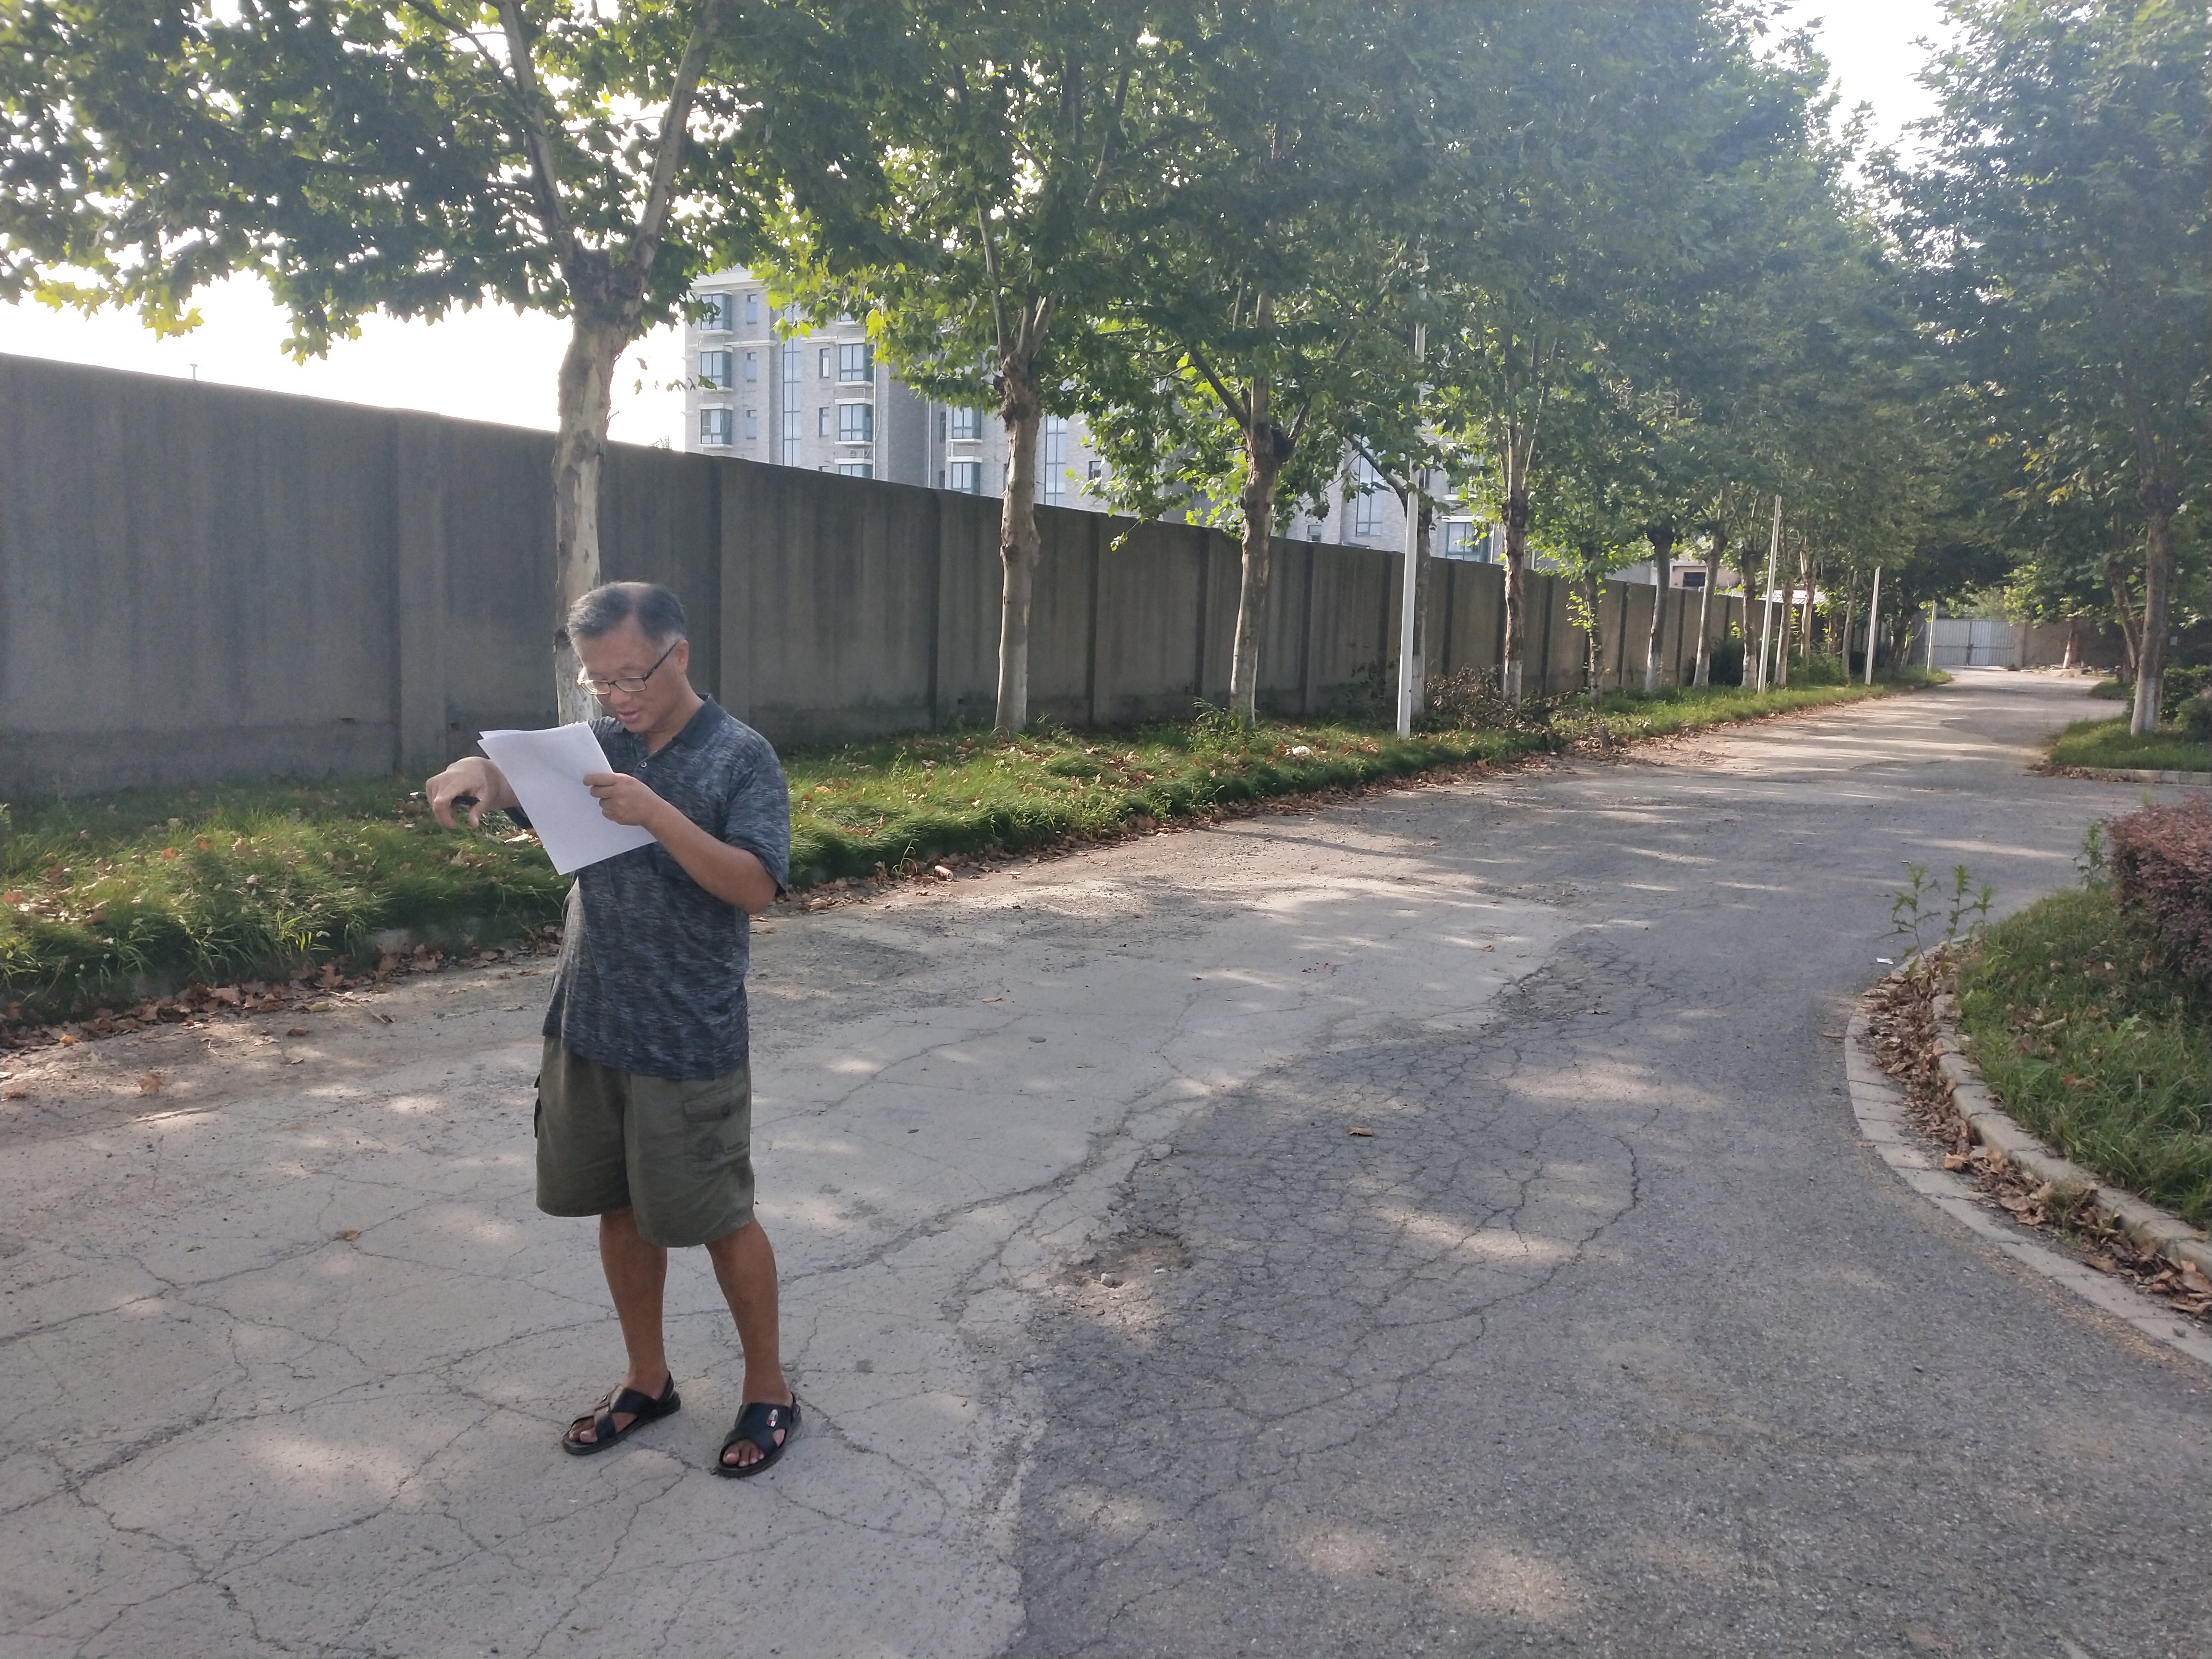
\includegraphics[
      width = \linewidth,
    ]{network/1}
    \caption{网口选择界面}%
    \label{fig:network/1}
  \end{subfigure}
  \quad
  \begin{subfigure}[htbp]{0.45\linewidth}
    \centering
    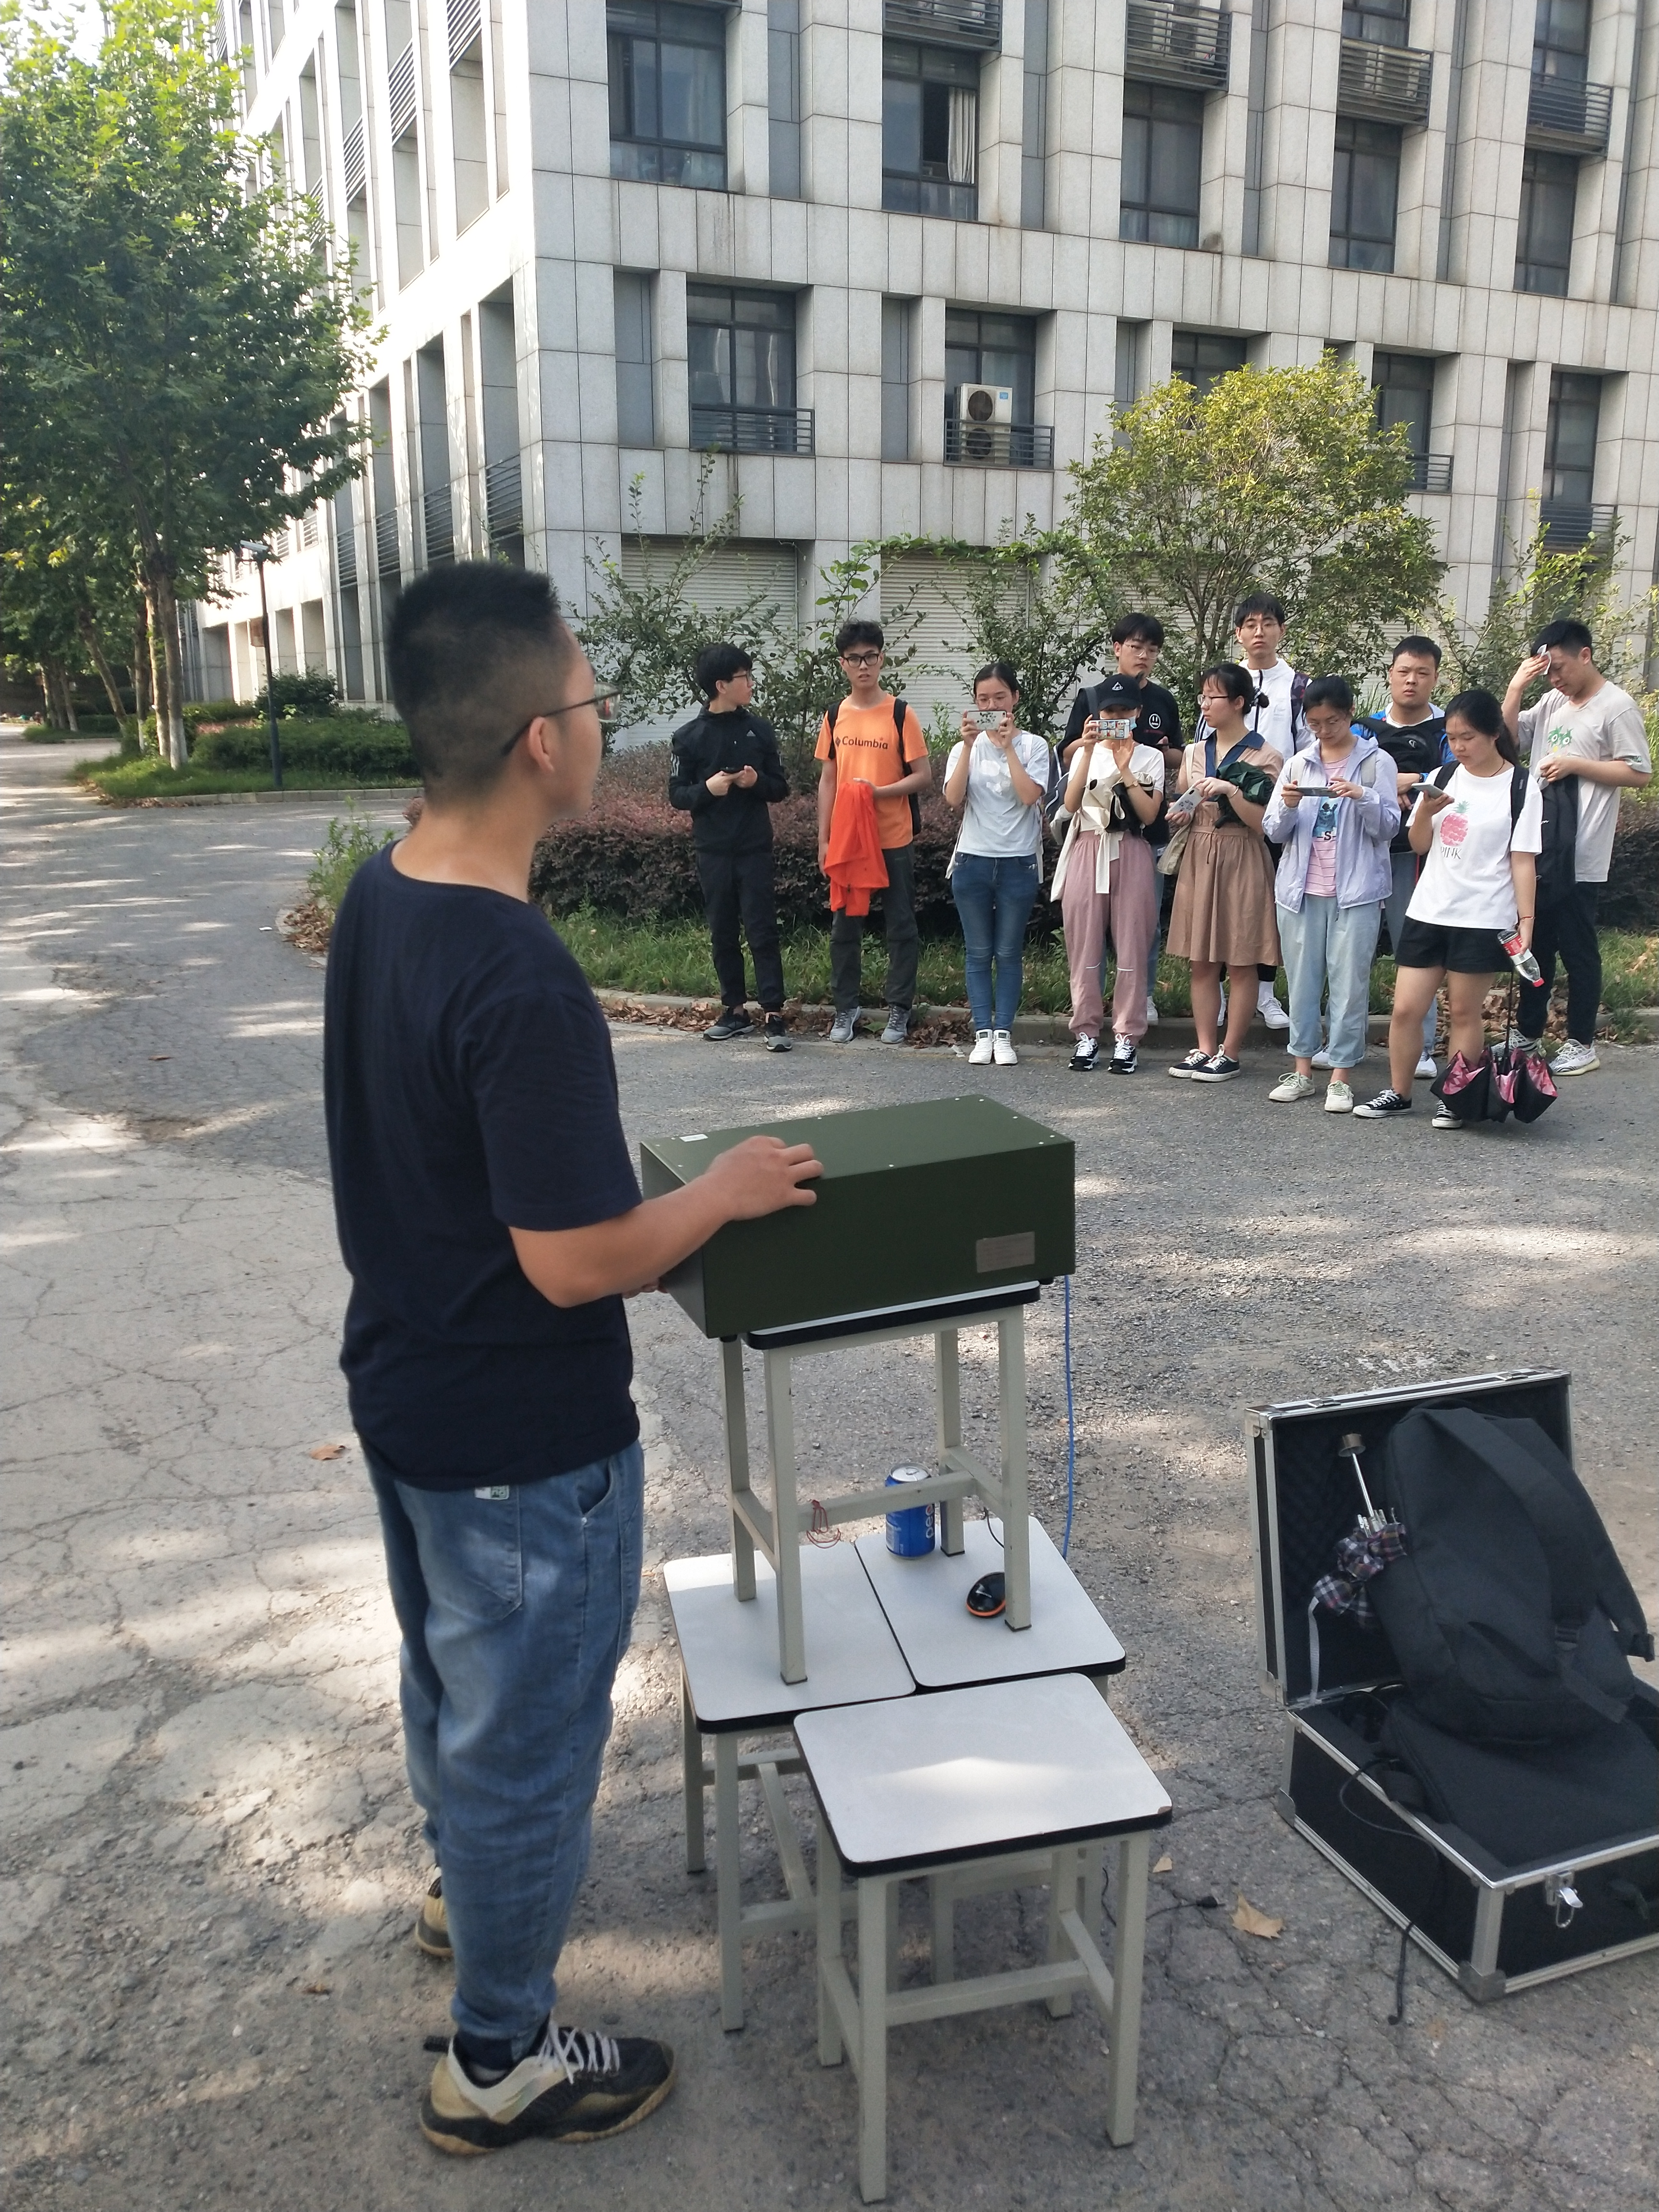
\includegraphics[
      width = \linewidth,
    ]{network/2}
    \caption{网卡选择提示界面}%
    \label{fig:network/2}
  \end{subfigure}
  \caption{网卡选择}%
  \label{fig:network}
\end{figure}

\begin{figure}[htbp]
  \centering
  \includegraphics[
    width = 0.6\linewidth,
  ]{software}
  \caption{上位机主界面}%
  \label{fig:software}
\end{figure}

\begin{table}[htbp]
  \centering
  \caption{上位机主界面}%
  \label{tab:software}
  \csvautobooktabular{tab/software.csv}
\end{table}

\subsubsection{实测场景演示}%
\label{ssub:test}

测试场景实拍见图~\ref{fig:test}。

\begin{figure}[htbp]
  \centering
  \includegraphics[
    width = 0.6\linewidth,
  ]{test}
  \caption{测试场景实拍图}%
  \label{fig:test}
\end{figure}

\end{document}

